
\chapter{Analyse logicielle}
\label{AnaLog}
    \section{Étalonnage de caméra}
    
\begin{figure}[H]
    \centering
    \subfloat[Image originale]{
        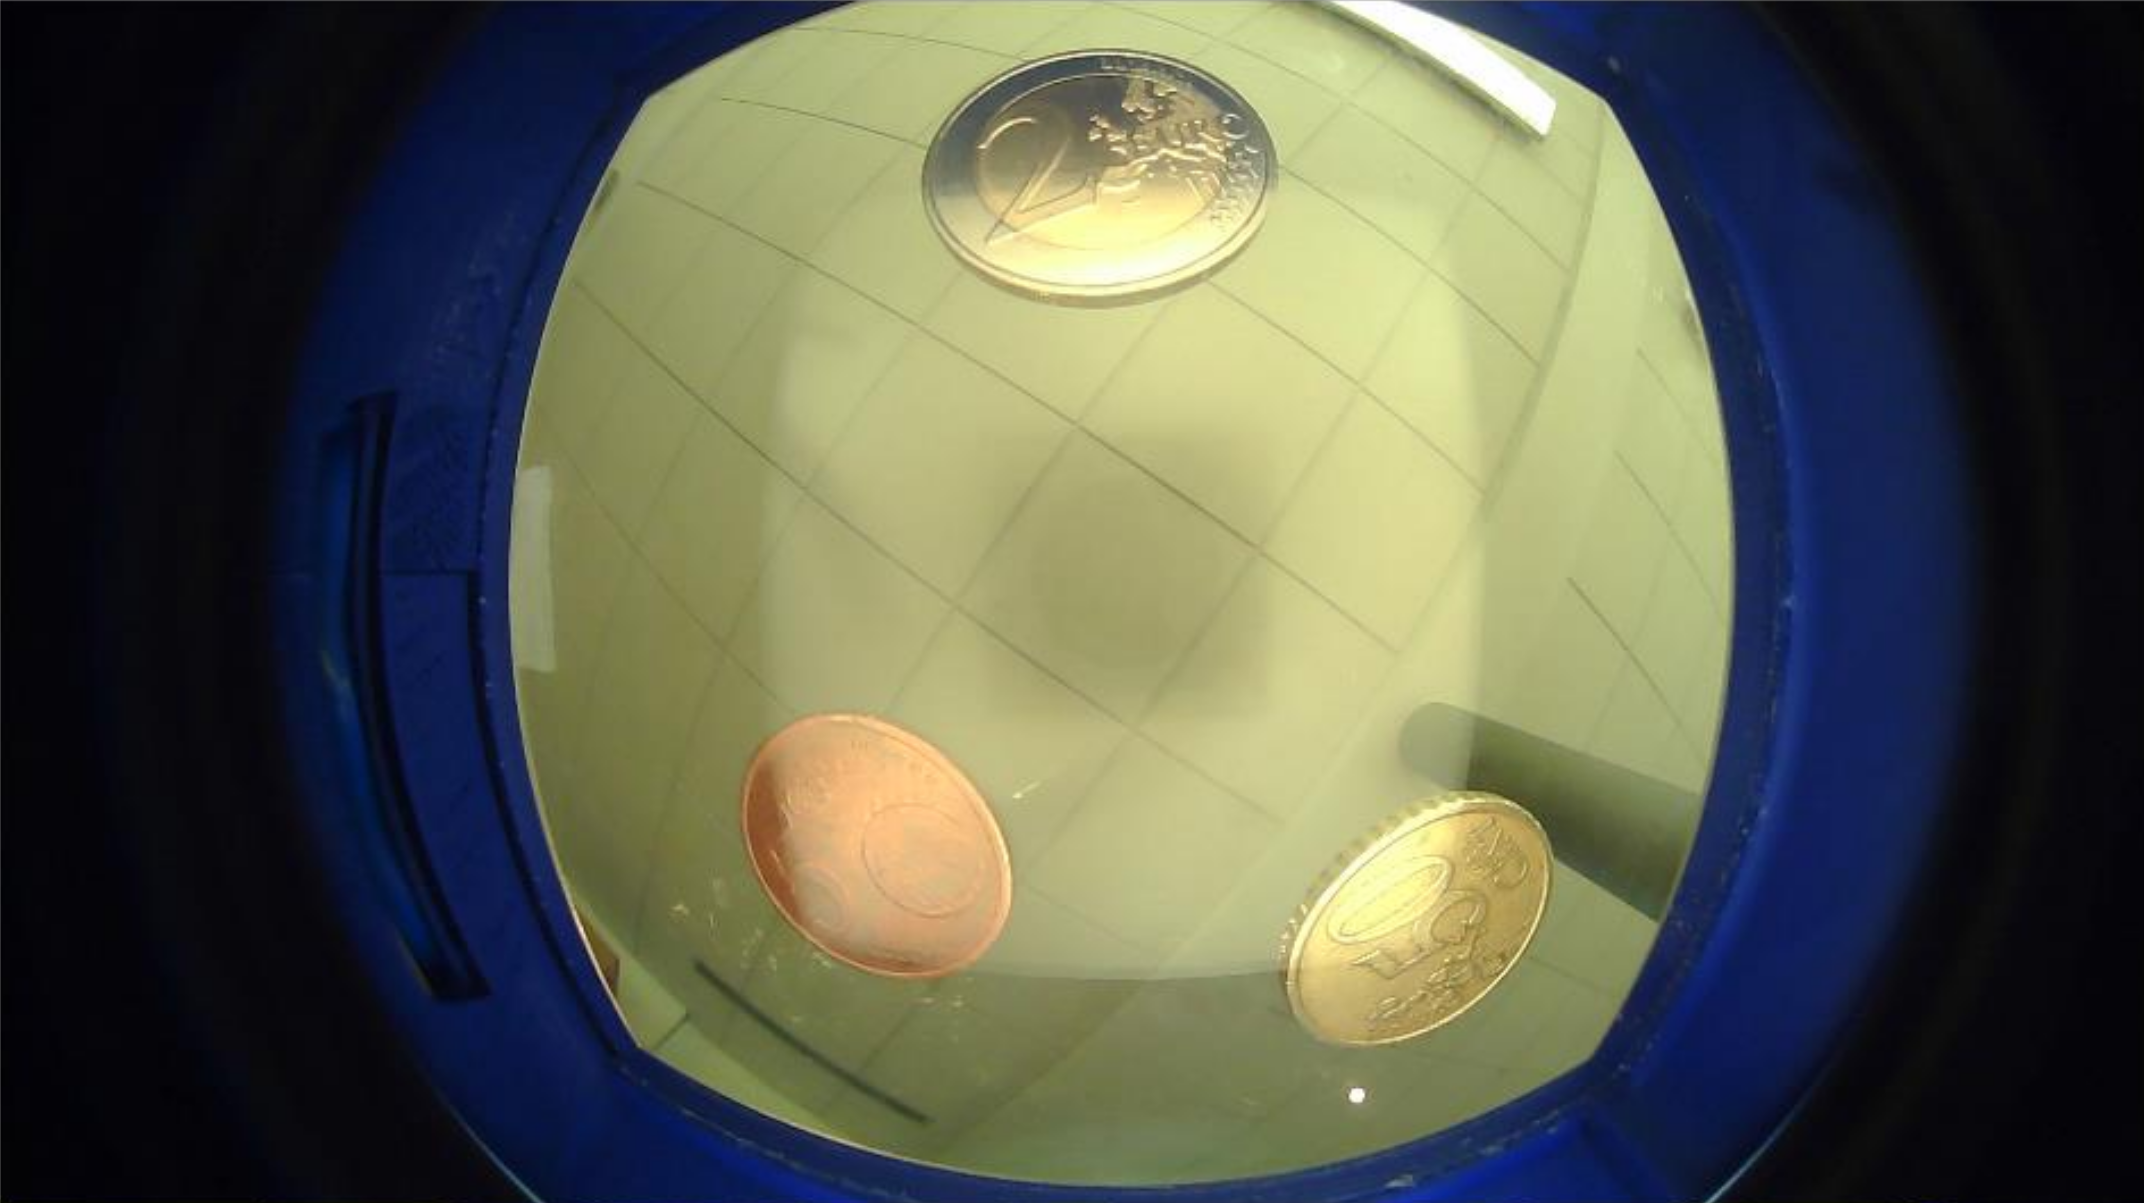
\includegraphics[width=0.6\textwidth]{img/Calibration_Original}
        \label{Calibration_Original}
    }
    \qquad
    \subfloat[Image de référence pour la calibration]{
        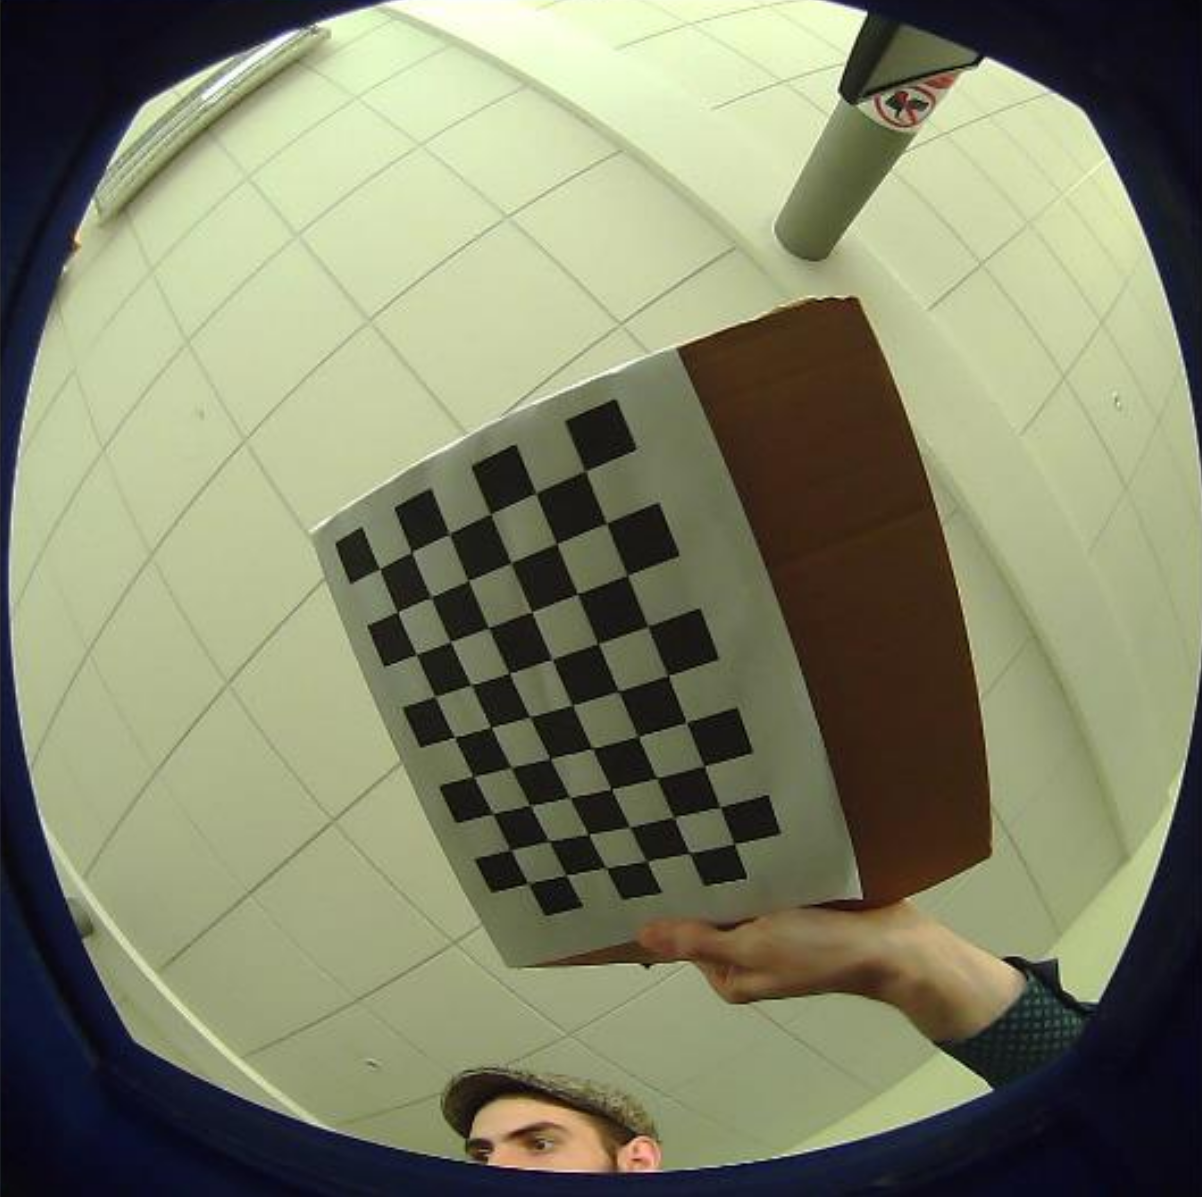
\includegraphics[width=0.4\textwidth]{img/Calibration_Chessboard}
        \label{Calibration_Chessboard}
    }
    \subfloat[Image recalibré]{
        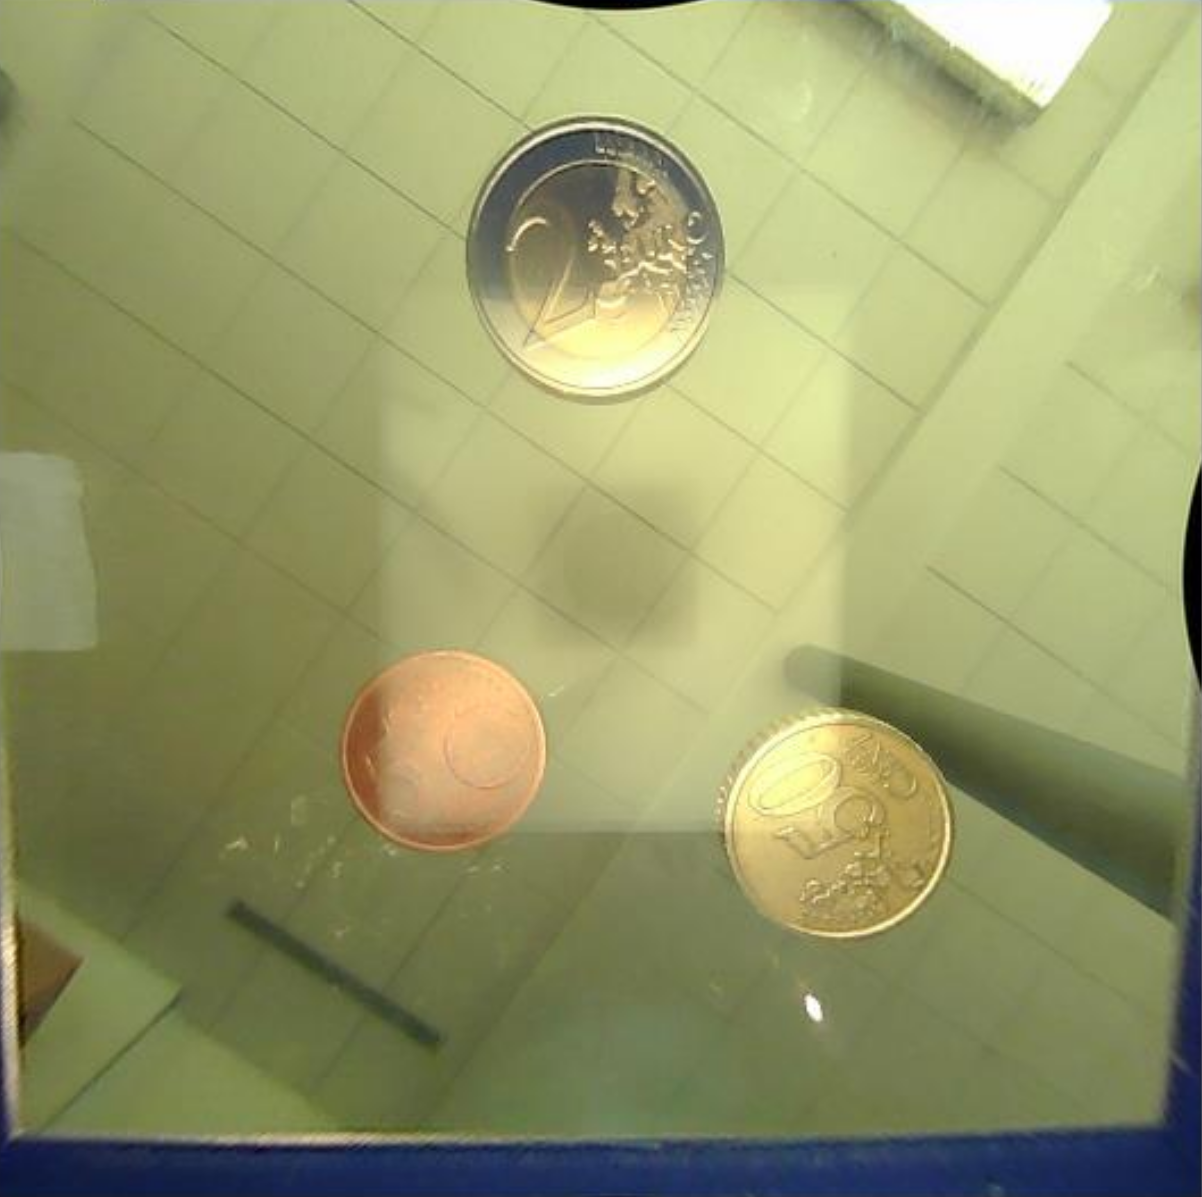
\includegraphics[width=0.4\textwidth]{img/Calibration_Undist}
        \label{Calibration_Undist}
    }
    \caption{Étalonnage de caméra}
    \label{CameraCalib}
\end{figure}

Avant l'opération de calibration de caméra, une première étape de recadrage est nécessaire.
À partir de l’image brute de 1920x1080p est faite une image carrée de 1080 pixels de côtés centrés sur la plaque.
La deuxième action est le remapage de l’image afin de corriger les problèmes de déformations géométriques causés par l’objectif.
La Figure \ref{CameraCalib} montre le résultat de cette calibration.
Pour calculer les coefficients de distorsions de la caméra, OpenCV fournit des fonctions utilitaires permettant de les calculer à partir d’un set d’images contenant un motif de géométrie connu (ici, un damier).
Le modèle du sténopé (aussi appelé modèle \emph{pin-hole}) n'est pas utilisé ici, on lui préférera le modèle dit \emph{fish-eye} ( les détails sont disponibles sur \url{http://docs.opencv.org/3.2.0/db/d58/group__calib3d__fisheye.html}).

    
    \section{Segmentation}
    
La segmentation d'image est une opération de traitement d'images qui a pour but de
rassembler des pixels entre eux suivant des critères prédéfinis.
Les pixels sont ainsi regroupés en régions, qui constituent un pavage ou une partition de l'image.
Il peut s'agir par exemple de séparer les objets du fond.

\begin{figure}[H]
    \centering
    \subfloat[Différence absolue]{
        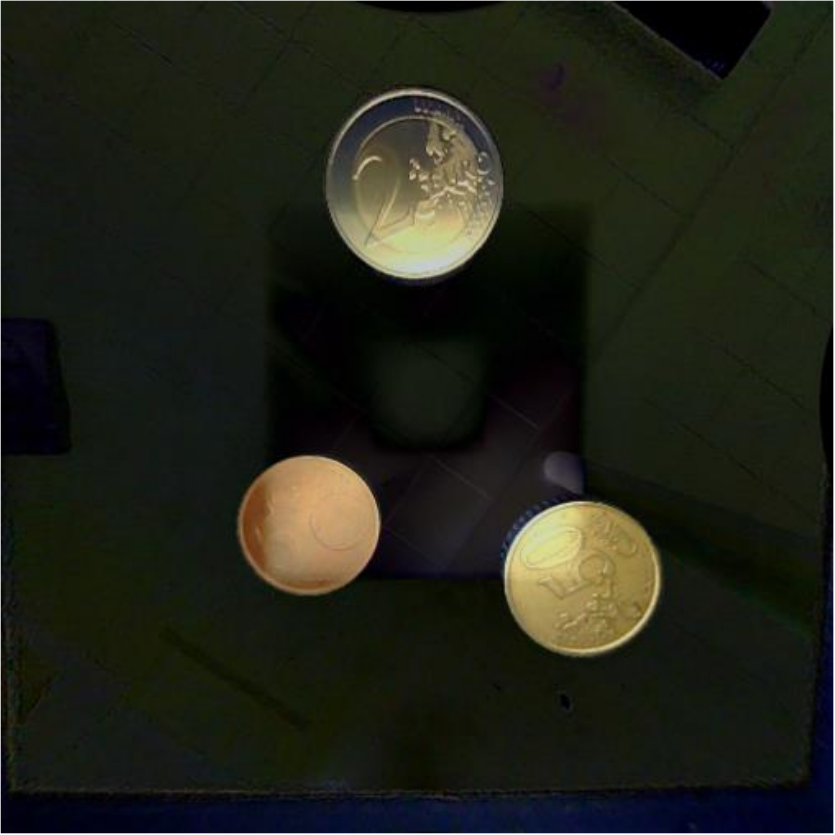
\includegraphics[width=0.3\textwidth]{img/Segmentation_AbsDiff}
        \label{Segmentation_AbsDiff}
    }
    \subfloat[Canal de teinte flouté]{
        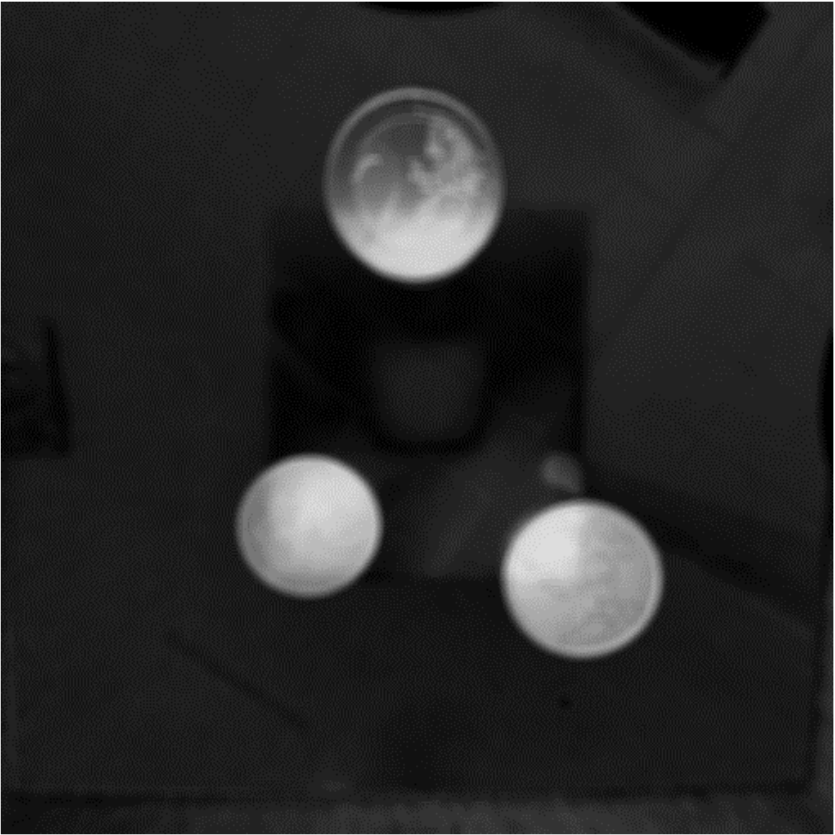
\includegraphics[width=0.3\textwidth]{img/Segmentation_HueBlurred}
        \label{Segmentation_HueBlurred}
    }
    \subfloat[Seuillage]{
        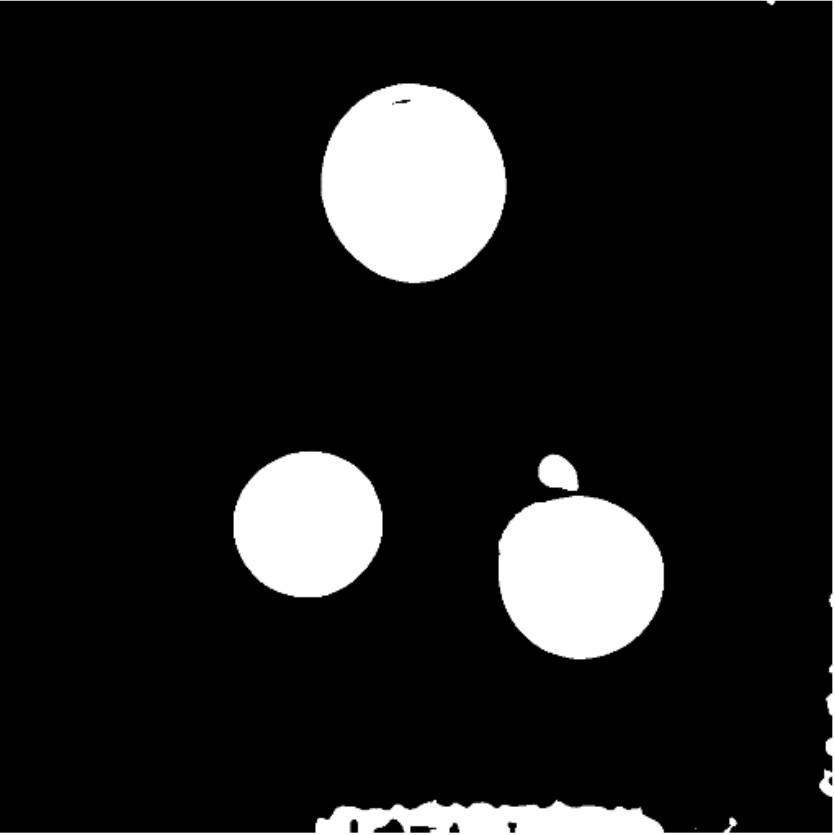
\includegraphics[width=0.3\textwidth]{img/Segmentation_Threshold}
        \label{Segmentation_Threshold}
    }
    \qquad
    \subfloat[Érosion]{
        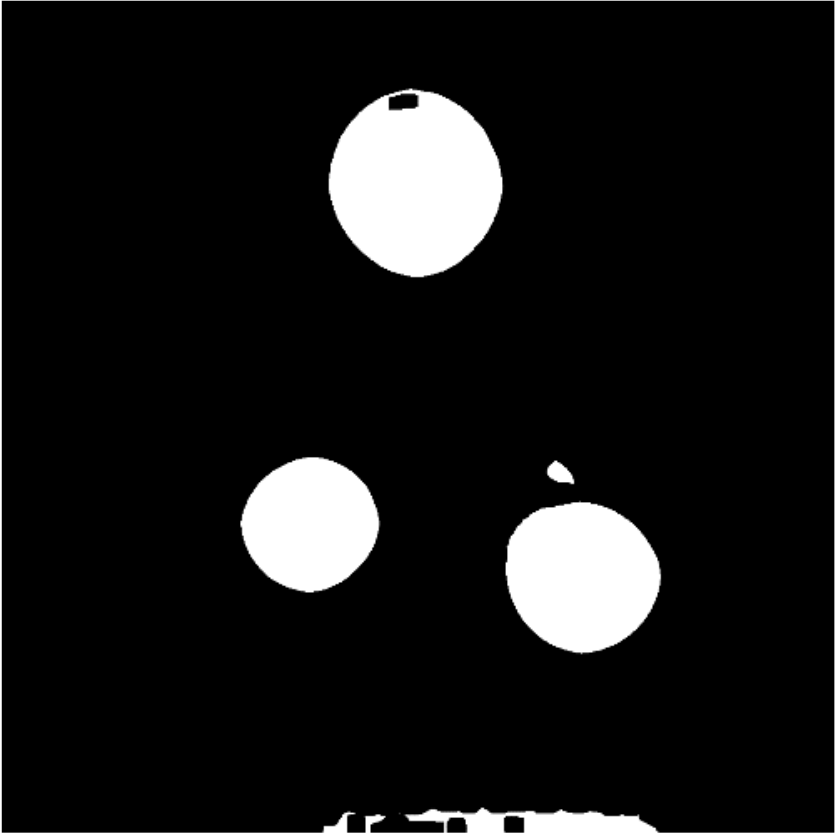
\includegraphics[width=0.3\textwidth]{img/Segmentation_Erosion}
        \label{Segmentation_Erosion}
    }
    \subfloat[Dilatation]{
        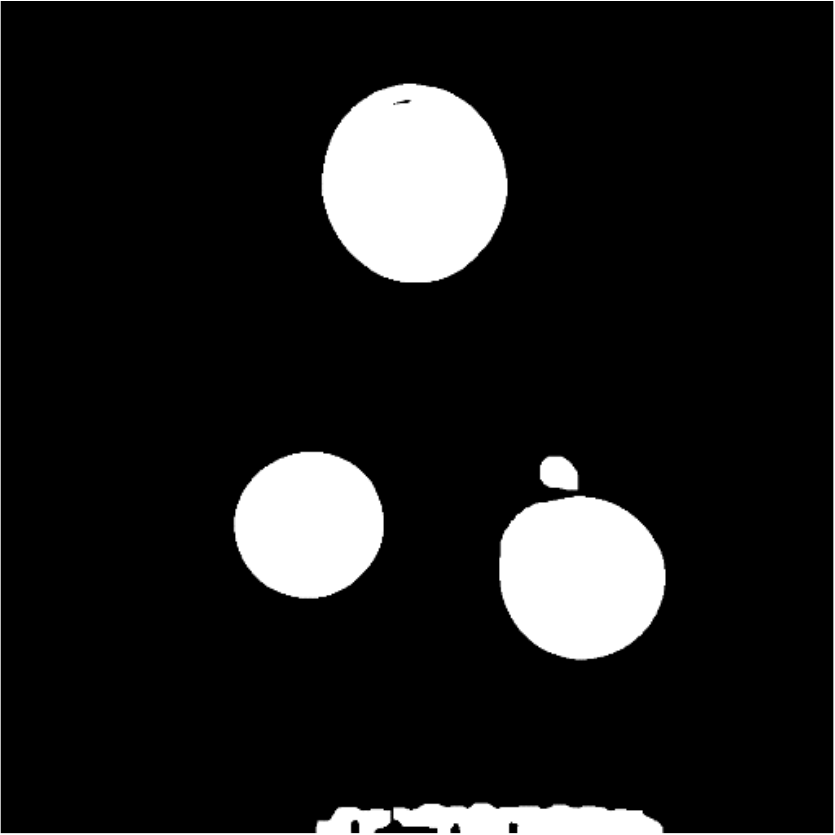
\includegraphics[width=0.3\textwidth]{img/Segmentation_Dilatation}
        \label{Segmentation_Dilatation}
    }
    \subfloat[Rectangles circonscrit]{
        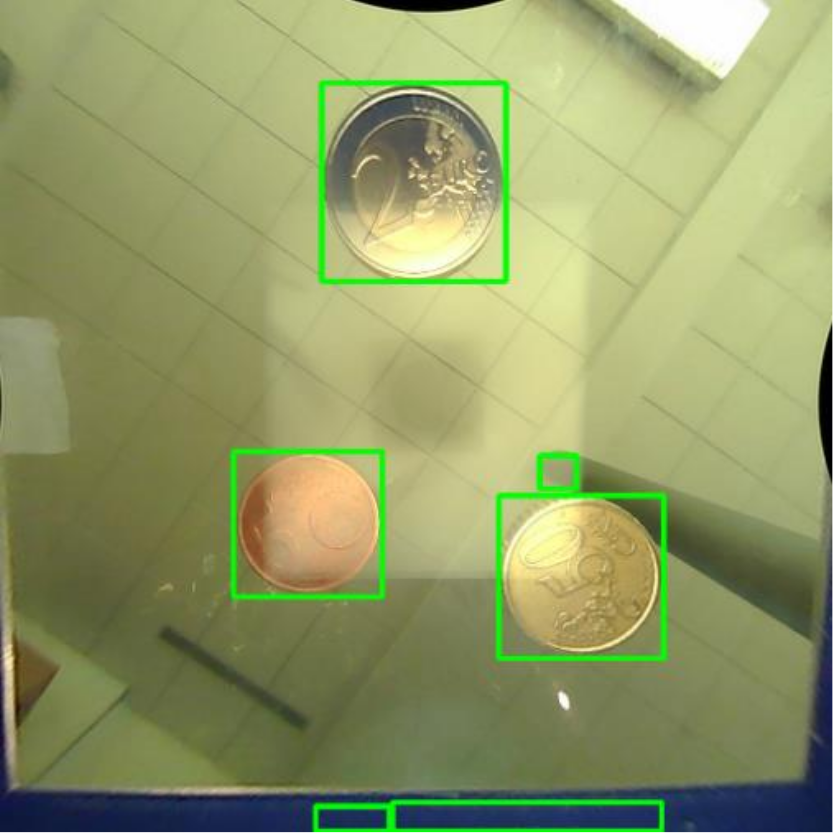
\includegraphics[width=0.3\textwidth]{img/Segmentation_BoundRect}
        \label{Segmentation_BoundRect}
    }
    \caption{Processus de segmentation}
    \label{segfig}
\end{figure}

Pour la Or-Box le pipeline de segmentation est assez simple.
Une fois les deux images obtenues, une avec éclairage et l’autre sans, on effectue les opérations suivantes :

\begin{itemize}
    \item On effectue la différence absolue des deux images, voir Figure \ref{Segmentation_AbsDiff}.
    \item On recode l’image obtenue en HSV (Hue / Saturation / Value) pour n’utiliser que le canal de valeur, car c’est dans celles-ci qu’est contenue l’information de luminosité pour chaque pixel.
    \item On floute le canal de valeur, en effectuant une convolution avec un noyau gaussien par exemple, voir Figure \ref{Segmentation_HueBlurred}.
    Cette étape n’est nécessaire que pour éviter un maximum de bruit lors de l’étape de seuillage suivante.
    \item L’étape de \emph{thresholding} (seuillage) consiste à appliquer la règle suivante pour chaque pixel :

\begin{absolutelynopagebreak}
    \begin{algorithmic}
    \If {$valeur \ge maxval$}
        \State $valeur \gets valeur_{max}$
    \Else
            \State $valeur\gets valeur_{min}$
    \EndIf
    \end{algorithmic}
\end{absolutelynopagebreak}

    Il ne reste plus qu’à trouver la valeur de seuil adapté.
    Il existe des méthodes de calcul de ce seuil basé sur les histogrammes –-- nous en avons utilisé principalement deux, soit la méthode d’Otsu \cite{otsu1975threshold} ou soit la méthode du triangle.
    
    Ces méthodes de segmentation avec un seuil globale ne marchent que si l’on suppose que l’histogramme de l’image est bimodal, c’est-à-dire qu’il existe deux piques d’intensité, un représentant les objets en premier plan et le second l’arrière-plan. Le résultat est visible sur la Figure \ref{Segmentation_Threshold}.
    \item Les opérations suivantes, l’érosion et la dilatation sont deux opérations morphologiques de base.
    Ces deux étapes servent à éliminer les régions blanches les plus petites, et à rassembler les plus proches en une seule plus grandes.
    \item La dernière étape consiste à trouver les contours des régions blanches, et trouver les rectangles circonscrits à ces contours, en vert sur la Figure \ref{Segmentation_BoundRect}.
    On effectuera ensuite le calcul des descripteurs et la classification seulement pour chacune des régions trouvées.
\end{itemize}
    
    \section{Classification automatique}
        \subsection{Définition formelle de la problématique}
        
        Formellement, le problème de la reconnaissance de forme dans un contexte d'apprentissage supervisé peut-être formulé ainsi :
        
        On considère la fonction inconnue $g:\mathcal{X}\rightarrow\mathcal{Y}$ qui définit pour chaque instance $\boldsymbol{x} \in \mathcal{X}$ en entrée, une étiquette $\boldsymbol{y} \in \mathcal{Y}$ en sortie .
        À partir des données d'entraînement $\mathbf{D} = \{(\boldsymbol{x}_1,y_1),\dots,(\boldsymbol{x}_n, y_n)\}$ que l'on considère comme étant des exemples corrects du passage entre les deux espaces, le but est de produire une fonction $h:\mathcal{X}\rightarrow\mathcal{Y}$ qui se rapproche le plus fidèlement possible de la fonction de mappage $g$.
        Le terme "le plus fidèlement possible" est défini en théorie de la décision grâce à une fonction de coût, le but alors est de minimiser cette fonction de coût durant la phase d'apprentissage.
        Dans la pratique on ne connait ni la distribution de $\mathcal{X}$ ni la fonction véritable fonction $g:\mathcal{X}\rightarrow\mathcal{Y}$.
        La seule solution est donc de collecter un grand nombre d'échantillon issu de $\mathcal{X}$ et de les étiquetés à la main avec la valeur de $\mathcal{Y}$ correcte.
        La procédure d'entraînement et de test utilisé pour la Or-Box est décrite dans la section \ref{protocoleExp}.
        
        Dans notre problème, $\boldsymbol{x}_i$ est la représentation d'une image d'un objet posé sur la vitre et $\boldsymbol{y}$ une des étiquettes parmi "un centime", "deux centimes", "cinq centimes", etc\dots
        On parle ici de "représentation d'une image" est non de l'image en entière.
        En effet, utiliser l'image brute comme ensemble $\mathcal{X}$ conduirait à une fonction $g:\mathcal{X}\rightarrow\mathcal{Y}$ extrêmement complexe à approximer.
        Il faut donc trouver un moyen intelligent de représenter l'image afin de réduire l'espace $\mathcal{X}$.
        On parle donc de descripteurs d'images (voir section  \ref{imgDescriptors}), il s'agit d'une fonction écrite par des experts du domaine qui prend l'image brute est la décrit en terme plus simple (couleurs, textures, contours, etc\dots). 
        
        \subsection{K plus proches voisins}
        
        La méthode des K plus proches voisins est une méthode d’apprentissage supervisé.
        Elle peut être utilisé dans des problèmes de classification et de régression.
        Dans les deux cas la sortie va dépendre des $k$ échantillons de la base d'apprentisage les plus proches dans l'espace de recherche.
        Dans le cas qui nous intéresse --- le problème de classification --- la sortie est l'appartenance a une classe. 
        Un object est classifié par un vote à la majorité de ses voisins, l'objet se voit assigné à la classe la plus courante parmi ces $k$ voisins.
        Le voisinage est définie par une fonction de distance, généralement une distance euclidienne ce qui sera aussi notre cas.
        
        Les perfomances d'un classificateurs peuvent parfois être améliorer en effectuant une transformation préalable sur chacune des caractéristiques.
        Deux transformation courrantes sont la \emph{standardization} et la \emph{fuzzification} \cite{peterson2009k}.
        
\begin{figure}[H]
    \centerline{
        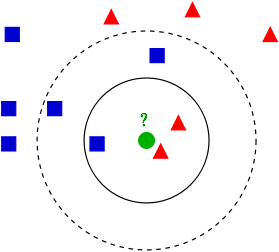
\includegraphics[width=0.35\textwidth,fbox]{img/Knn_Example}
    }
    \caption{Exemple pour classification avec K plus proches voisins - Auteur: Antti Ajanki}
    \label{KNNpic}
\end{figure}

        Dans l'exemple de la figure \ref{KNNpic}, l'échantillon à classé est représenté en vert, l'espace de recherche est à deux dimension et la base d'apprentissage contient des échantillons appartenant à deux classes, une rouge et une bleu.
        Si on choisi $k=3$ alors le cercle vert sera classé comme appartenant à la même classe que les triangles rouge, alors que pour $k=5$ il sera classé appartenant à la classe des carrés bleus.
        
        
        \subsection{Machine à vecteurs de support}
        
        Tout comme les KNN les SVM servent à résoudre des problème de classification et de régréssion.
        Cependant contrairement à ce premier ce n'est pas un algorithme \emph{lazy learning}, c'est à dire qu'il n'attend pas une requête pour essayer de généralisé les donnés d'apprentissage.
        
        Le premier problème que résout les SVM est celui de trouver une frontière séparant de manière optimale l'espace de recherche à partir de la base d'apprentissage.
        Cette frontière est un hyperplan dont la marge est maximale, c'est à dire que l'on cherche a maximiser la distance entre la frontière de séparation et les échnatillons les plus proches.
        
        Le deuxième problème que résout les SVM est celui de traiter les données qui ne sont pas linéairement séparables.
        Pour cela on cherche a paser dans un espace de plus grande dimension dans le quelle il est probable de trouver un séparation linéaire.
        Plus formellement, on applique aux vecteurs d'entrée x une transformation non-linéaire $\phi$.
        L'espace d'arrivée$\phi (X)$ est appelé espace de redescription dans lequel on peut reformuler notre recherche d'optimisation de marge.
        Cette reformulation fait apparaîtres des produits scalaires dans un espace à dimension élevée ce qui est très coûteux en terme de calcul.
        On fait alors appelà la méthode du \emph{kernel trick} qui utilise une fonction noyau pour rester dans l'espace d'origine.
        La fonction noyau doit respecter certain condition comme celle de correspondre à un produit scalaire dans un espace de grande dimension.
        
        
        \subsection{Protocole d'évaluation expérimentale}

        Chaque méthode de classification devra être testé sur l'ensemble des huit classes de pièces.
        La validité du modèle sera validé par validation croisé en \emph{"k-fold cross validation"} \cite{Refaeilzadeh2009}.
        Cette méthode consiste a diviser les échantillons originaux en $k$ sous-ensembles, puis a sélectionner l'un des $k$ sous-ensemble d'échantillons comme ensemble de validation et les ($k-1$) autres sous-ensembles constitueront l'ensemble d'apprentissage.
        On calcul l'erreur de prédiction pour l'ensemble de validation --- soit nombre d'échantillons dont la classe a été incorrectement prédit sur le nombre total d'échantillon de l'ensemble de validation.
        Puis on répète $k$ fois l'opération en sélectionnant un autre ensemble de validation parmi les ($k-1$) sous-ensembles qui n'ont pas encore été utilisés.
        Ainsi chaque échantillon a été utilisé exactement une fois comme ensemble de validation.
        L'erreur de prédiction total pour cette méthode est la moyenne des $k$ taux de prédiction.
        
        

    \section{Description d'image}
    \label{imgDescriptors}
        \subsection{Color-based descriptor}
        Une première approche pour distingué les différentes classes de pièces est de se basé sur leurs couleurs.
        Pour décrire une image par sa couleur --- ou ses couleurs --- on peut calculer son histogramme. 
        Afin de se prémunir au maximum des variations d'éclairage nous calculerons l'histogramme du canal \emph{Hue}.
        Puisque seul la distribution entre ces valeurs nous intéresse, nous les normaliserons entre 0 et 255.
        
        La figure \ref{Hists} montre les histogrammes moyens obtenues sur l'ensemble des échantillons de trois classe; la ligne bleu représente la valeur moyenne et la zone grise l'intervalle de confiance à un écart-type.
        On remarque que ces trois histogrammes sont mono-mode, que les pièces rouges ont un mode centré autour de 15, que les pièces jaunes et celles de un et deux euros ont un mode centré autour de 20.
        
\begin{figure}[H]
    \centering
    \subfloat[Pièces de un centime]{
        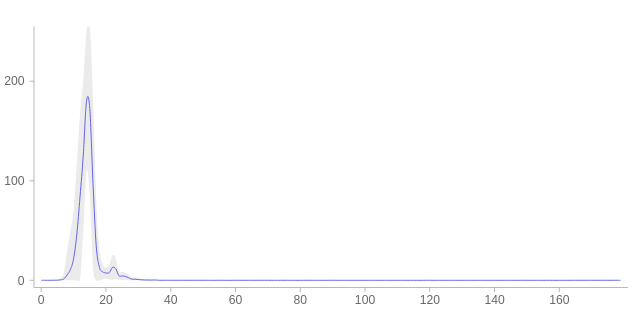
\includegraphics[width=0.6\textwidth]{img/OneCentHist}
        \label{HistOneCent}
    }
        \qquad
    \subfloat[Pièces de dix centimes]{
        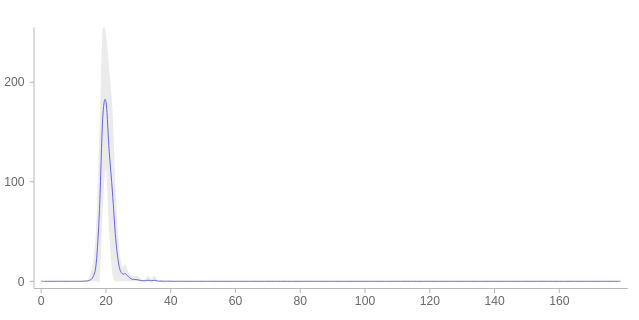
\includegraphics[width=0.6\textwidth]{img/TenCentHist}
        \label{HistTenCent}
    }
        \qquad
    \subfloat[Pièces de un euro]{
        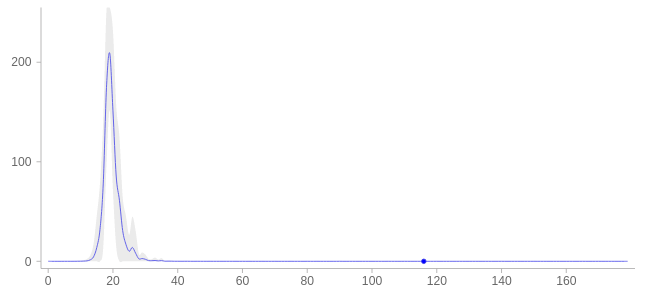
\includegraphics[width=0.6\textwidth]{img/OneEuroHist}
        \label{HistEuro}
    }
    \caption{Histogrammes moyen}
    \label{Hists}
\end{figure}
        
        \subsection{Shape-based descriptors}
        
        La distinction par couleur ne suffisant pas à distinguer les catégories entre elles, nous calculerons aussi les descripteurs suivants :
        \begin{description}
            \item[Le périmètre] du contour
            \item[L'aire]
            \item[La circularité]
            \item[Largeur du rectangle circonscrit d'aire minimum]
            \item[Hauteur du rectangle circonscrit d'aire minimum]
        \end{description}
        
        Pour chacune de ces caractéristiques ont été calculé la moyenne et l'écart-type afin de savoir si il serait potentiellement exploitable 
        
        \subsection{Binary descriptors}
        Suivant les résultats obtenues et le temps restant sur le projet des descripteurs plus complexes que ceux mentionnés ci-dessus.
        L'utilisation de ces types de descripteurs bien que très puissants et générique n'est pas une priorité pour ce projet.
        En effet, lors du projet collectif de quatrième année se sont ces méthodes qui ont était testé avec des résultats décevants --- \~30\% d'erreur.
        La faute au manque de contraste des textures visibles sur les pièces du à redéformation sur les bord de l'image.
        
 
% \nocite{*} % make all bib ref appear even if not cited
\bibliographystyle{alpha}
\bibliography{mybib}


    
        